\documentclass[tikz,border=15pt]{standalone}
\usepackage{tikz}
\usepackage{amsmath}
\usepackage{amssymb}
\usetikzlibrary{shapes.geometric, arrows.meta, positioning, calc, backgrounds, fit, shadows.blur}

\definecolor{navyDark}{HTML}{0B2545}
\definecolor{navyLight}{HTML}{F0F4F8}
\definecolor{navyBorder}{HTML}{134074}

\definecolor{emeraldDark}{HTML}{0E6251}
\definecolor{emeraldLight}{HTML}{E8F8F5}
\definecolor{emeraldBorder}{HTML}{16A085}

\definecolor{purpleDark}{HTML}{512E5F}
\definecolor{purpleLight}{HTML}{F4ECF7}
\definecolor{purpleBorder}{HTML}{8E44AD}

\definecolor{amberDark}{HTML}{7D6608}
\definecolor{amberLight}{HTML}{FEF9E7}
\definecolor{amberBorder}{HTML}{D4AC0D}

\definecolor{crimsonDark}{HTML}{78281F}
\definecolor{crimsonLight}{HTML}{FDF2E9}
\definecolor{crimsonBorder}{HTML}{C0392B}

\definecolor{slateDark}{HTML}{2C3E50}
\definecolor{slateLight}{HTML}{F8F9FA}
\definecolor{slateBorder}{HTML}{BDC3C7}

\begin{document}
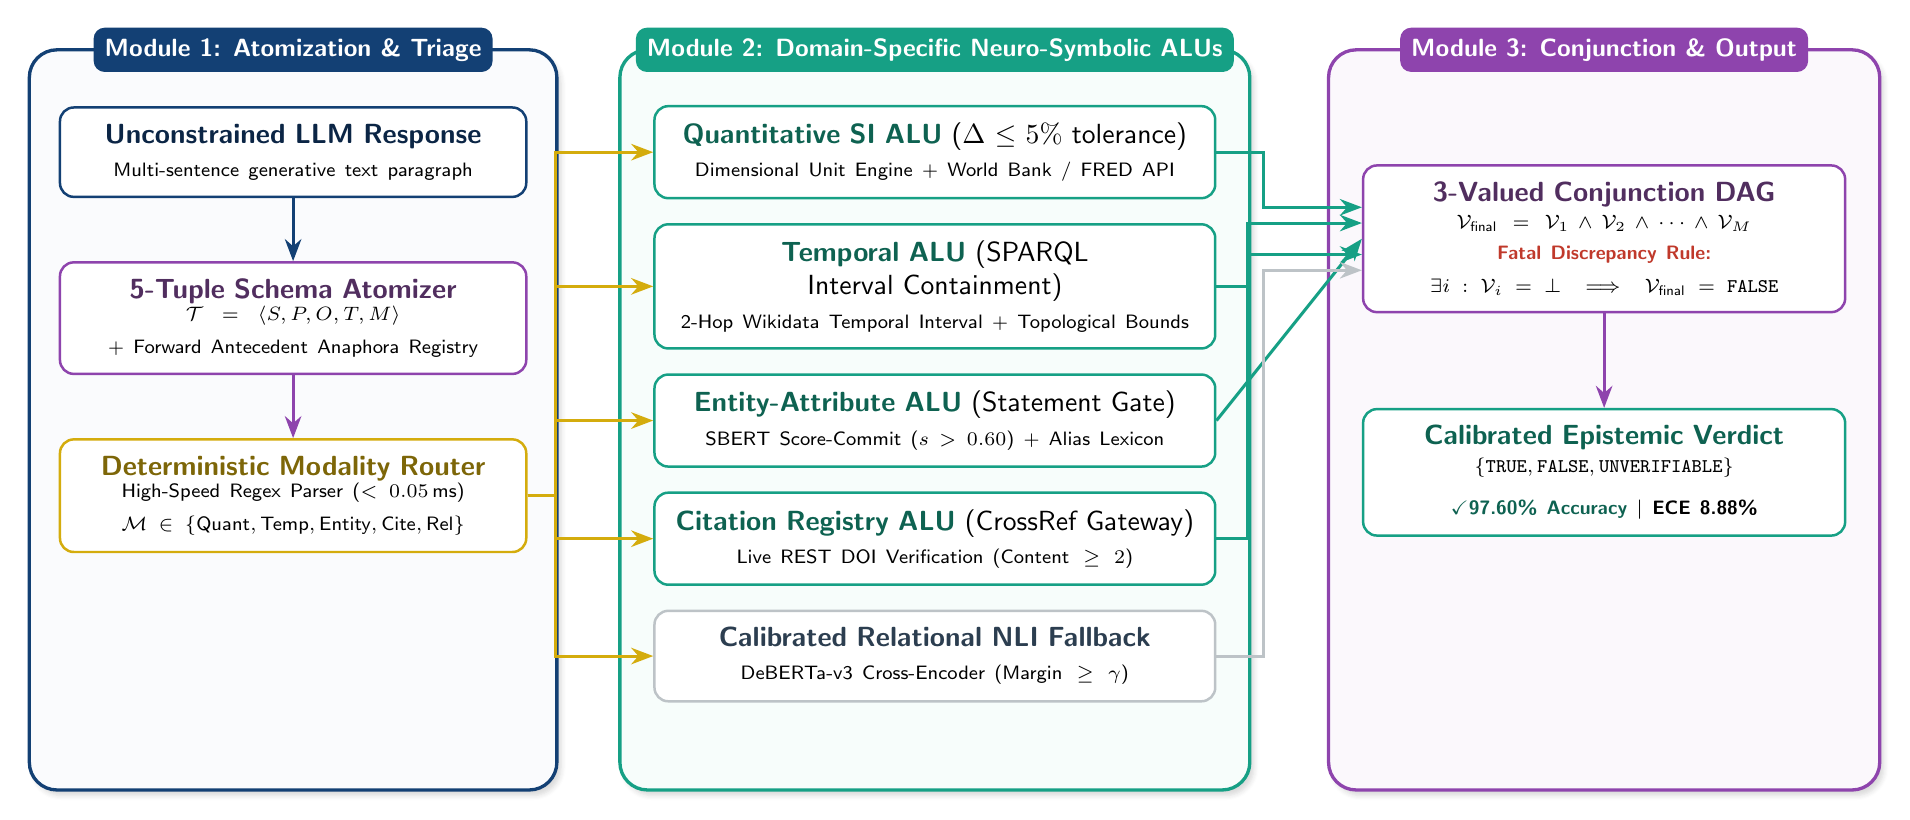
\begin{tikzpicture}[
    font=\sffamily,
    >=Stealth,
    modulebox/.style={
        draw=#1Border, fill=#1Light!35, line width=1.2pt, rounded corners=10pt,
        blur shadow={shadow blur steps=5, shadow xshift=1.5pt, shadow yshift=-2pt, shadow opacity=15}
    },
    card/.style={
        draw=#1Border, fill=white, line width=0.9pt, rounded corners=5pt,
        align=center, inner sep=6pt
    },
    wire/.style={
        ->, line width=1.1pt, draw=#1Border
    }
]

% ==================== MODULE 1 ====================
\draw[modulebox=navy] (-0.3, -5.8) rectangle (6.4, 3.6);
\node[fill=navyBorder, text=white, font=\bfseries\sffamily\small, rounded corners=4pt, inner sep=4pt] at (3.05, 3.6) {Module 1: Atomization \& Triage};

\node[card=navy, minimum width=5.8cm, text width=5.5cm] (m1_in) at (3.05, 2.3) {
    \textbf{\color{navyDark} Unconstrained LLM Response}\\
    \scriptsize Multi-sentence generative text paragraph
};

\node[card=purple, below=0.8cm of m1_in, minimum width=5.8cm, text width=5.5cm] (m1_atom) {
    \textbf{\color{purpleDark} 5-Tuple Schema Atomizer}\\
    \scriptsize $\mathcal{T} = \langle S, P, O, T, M \rangle$\\
    \scriptsize + Forward Antecedent Anaphora Registry
};

\node[card=amber, below=0.8cm of m1_atom, minimum width=5.8cm, text width=5.5cm] (m1_router) {
    \textbf{\color{amberDark} Deterministic Modality Router}\\
    \scriptsize High-Speed Regex Parser ($<0.05\,\text{ms}$)\\
    \scriptsize $\mathcal{M} \in \{\text{Quant}, \text{Temp}, \text{Entity}, \text{Cite}, \text{Rel}\}$
};

\draw[wire=navy] (m1_in) -- (m1_atom);
\draw[wire=purple] (m1_atom) -- (m1_router);

% ==================== MODULE 2 ====================
\draw[modulebox=emerald] (7.2, -5.8) rectangle (15.2, 3.6);
\node[fill=emeraldBorder, text=white, font=\bfseries\sffamily\small, rounded corners=4pt, inner sep=4pt] at (11.2, 3.6) {Module 2: Domain-Specific Neuro-Symbolic ALUs};

\node[card=emerald, minimum width=7.0cm, text width=6.7cm] (alu_q) at (11.2, 2.3) {
    \textbf{\color{emeraldDark} Quantitative SI ALU} ($\Delta \le 5\%$ tolerance)\\
    \scriptsize Dimensional Unit Engine + World Bank / FRED API
};

\node[card=emerald, below=0.3cm of alu_q, minimum width=7.0cm, text width=6.7cm] (alu_t) {
    \textbf{\color{emeraldDark} Temporal ALU} (SPARQL Interval Containment)\\
    \scriptsize 2-Hop Wikidata Temporal Interval + Topological Bounds
};

\node[card=emerald, below=0.3cm of alu_t, minimum width=7.0cm, text width=6.7cm] (alu_e) {
    \textbf{\color{emeraldDark} Entity-Attribute ALU} (Statement Gate)\\
    \scriptsize SBERT Score-Commit ($s > 0.60$) + Alias Lexicon
};

\node[card=emerald, below=0.3cm of alu_e, minimum width=7.0cm, text width=6.7cm] (alu_c) {
    \textbf{\color{emeraldDark} Citation Registry ALU} (CrossRef Gateway)\\
    \scriptsize Live REST DOI Verification ($\text{Content} \ge 2$)
};

\node[card=slate, below=0.3cm of alu_c, minimum width=7.0cm, text width=6.7cm] (alu_r) {
    \textbf{\color{slateDark} Calibrated Relational NLI Fallback}\\
    \scriptsize DeBERTa-v3 Cross-Encoder ($\text{Margin} \ge \gamma$)
};

% Router to ALU Connectors
\draw[wire=amber] (m1_router.east) -- ++(0.35,0) |- (alu_q.west);
\draw[wire=amber] (m1_router.east) -- ++(0.35,0) |- (alu_t.west);
\draw[wire=amber] (m1_router.east) -- ++(0.35,0) |- (alu_e.west);
\draw[wire=amber] (m1_router.east) -- ++(0.35,0) |- (alu_c.west);
\draw[wire=amber] (m1_router.east) -- ++(0.35,0) |- (alu_r.west);

% ==================== MODULE 3 ====================
\draw[modulebox=purple] (16.2, -5.8) rectangle (23.2, 3.6);
\node[fill=purpleBorder, text=white, font=\bfseries\sffamily\small, rounded corners=4pt, inner sep=4pt] at (19.7, 3.6) {Module 3: Conjunction \& Output};

\node[card=purple, minimum width=6.0cm, text width=5.7cm] (dag) at (19.7, 1.2) {
    \textbf{\color{purpleDark} 3-Valued Conjunction DAG}\\
    \vspace{2pt}
    \scriptsize $\mathcal{V}_{\text{final}} = \mathcal{V}_1 \wedge \mathcal{V}_2 \wedge \dots \wedge \mathcal{V}_M$\\
    \vspace{3pt}
    \scriptsize \textbf{\color{crimsonBorder} Fatal Discrepancy Rule:}\\
    \scriptsize $\exists i: \mathcal{V}_i = \bot \implies \mathcal{V}_{\text{final}} = \texttt{FALSE}$
};

\node[card=emerald, below=1.2cm of dag, minimum width=6.0cm, text width=5.7cm] (decision) {
    \textbf{\color{emeraldDark} Calibrated Epistemic Verdict}\\
    \vspace{2pt}
    \scriptsize $\{\texttt{TRUE}, \texttt{FALSE}, \texttt{UNVERIFIABLE}\}$\\
    \vspace{3pt}
    \scriptsize \textbf{\color{emeraldDark}\checkmark 97.60\% Accuracy} $|$ \textbf{ECE 8.88\%}
};

% Direct Parallel Clean Connections into DAG
\draw[wire=emerald] (alu_q.east) -- ++(0.6,0) |- ($(dag.west) + (0, 0.4)$);
\draw[wire=emerald] (alu_t.east) -- ++(0.4,0) |- ($(dag.west) + (0, 0.2)$);
\draw[wire=emerald] (alu_e.east) -- (dag.west);
\draw[wire=emerald] (alu_c.east) -- ++(0.4,0) |- ($(dag.west) - (0, 0.2)$);
\draw[wire=slate] (alu_r.east) -- ++(0.6,0) |- ($(dag.west) - (0, 0.4)$);

\draw[wire=purple] (dag) -- (decision);

\end{tikzpicture}
\end{document}
